% Chapter Template

\chapter{Working Environment} % Main chapter title

\label{Chapter2} % Change X to a consecutive number; for referencing this chapter elsewhere, use \ref{ChapterX}

\lhead{Chapter 2. \emph{Working Environment}} % Change X to a consecutive number; this is for the header on each page - perhaps a shortened title

%----------------------------------------------------------------------------------------
%	SECTION 1
%----------------------------------------------------------------------------------------

%http://www.cisco.com/web/FR/documents/pdfs/livres_blancs/mobilite_sans_fil/Protocole_LWAPP.pdf

\section{UCL's wireless infrastructure}

On its Louvain-la-Neuve's campus area, the Catholic University of Louvain offers five different networks, each with a different SSID, that are reserved to certain parts of users according to their category. Those available networks are the following:
\begin{itemize}
	\item[-] \texttt{student.UCLouvain}: Available for all the students enrolled at UCL.
	\item[-] \texttt{UCLouvain}: Reserved for university's professors and the researchers.
	\item[-] \texttt{UCLouvain-prive}: Limited access to check the UCL's wireless configuration page or to download required program for Windows XP and Vista.
	\item[-] \texttt{visiteurs.UCLouvain}: Accessible for guests invited by the university.
	\item[-] \texttt{eduroam}: International education roaming access.
\end{itemize}

Network security is an important issue and an everyday struggle at the university and several measures are regularly taken by the SRI team in order to keep the integrity and the consistency of the UCL's network preserved. As an example, Microsoft has decided on the 8th of April 2014 to end the Windows XP's support and updates leaving all the remaining laptops running this operating system unprotected to possible external threats\cite{windows}. The problem with that Microsoft's decision is that those outdated computers might become more vulnerable to security risks and malwares/viruses. It could become a real problem for the university's network because if a contaminated host is able to connect to the network it can cause serious damages to the overall infrastructure. In order to counter this possible problem, the SRI team took the decision to block the wireless access to any device that still uses Windows XP since the 8th of April.

The main way of protecting the network infrastructure from exterior threats that has been installed and configured by the SRI team is the use of the \texttt{IEEE 802.1X} standard providing an authentication mechanism for all the devices that want to connect to a UCL's wireless network. This architecture uses an authentication with user ID and password. Basically, every student, professor, researcher or staff members needs an username and a password in order to connect to one of the networks and get access to the Internet inside the UCL's campus. The username is composed of two parts, on one side the login the user has received from the university's administrative system when he enrolled himself, and on the other side the domain (for example \texttt{@wifi.uclouvain.be}). Along with that username, the user also needs a password. This password is the same as the password he uses to connect to his personal virtual office on the university's web site. Without those credentials it is impossible for him to connect to the UCL's wireless network.

This kind of authentication mechanism is only possible if the infrastructure has several key entities that are going to handle all this security authentication process. Those entities are an \textit{authentication server} and an \textit{authenticator}. Typically an authentication server is a host that supports the \texttt{RADIUS} and  \texttt{EAP} protocols. In the case of the UCL's infrastructure the authenticator is also composed of several database servers that support the \texttt{LDAP} (\textit{Lightweight Directory Access Protocol}) protocol where all the information about the students, professors, researchers and staff members of the UCL are stored. Among those stored data, there are all the users' credentials. The authenticator are the access points that handles the connection request from the user and a Cisco controller that handles all the authentication process. This authenticator is the real security guard for the network since the client is not allowed to access to the protected side of the network until it's identity has been validated and authorized.

Let's keep in mind that these controller and access points do not play in the real world of the authentication itself. They are called the \textit{Authenticator} because that is where the client asks for authentication but it do not authenticate the client. The device that authenticate the client is the \textit{Authentication Server}.

Also, there are two ways of authentication on the UCL's network. Either, the user wants to connect to the network using WiFi or he can use a wired connection to the network. Those two types of connection requires a different authentication process. For WiFi, the authentication process uses \texttt{IEEE 802.1X} protocol in addition with \texttt{EAP} while for wired connection, the process uses \texttt{RADIUS-MAC} authentication process. 


\section{WLAN authentication process}
Let's first analyze the authentication process mechanism with WiFi.
As explained before, with the \texttt{IEEE 802.1X} standard, there are two key parts, the \textit{Authenticator} and the \textit{Authentication Server}. In the case of a WiFi authentication process, a third one can be added to this list and is called the \textit{Supplicant}. The supplicant is simply the wireless client that asks for an authentication in order to have access to the protected network. The authentication process works in several key steps and uses different protocols.

First of all, the supplicant who wants to access the network needs to make a special request to the authenticator. During that step the protocols that are used between the supplicant and the authenticator are a combination of \texttt{802.1X} and \texttt{EAP} protocol (\textit{Extensible Authentication Protocol}). Thanks to \texttt{802.1X} protocol, the authenticator can refuse any access to the network as long as the authentication server has not authenticated the client and accepted to open the access (i.e. open the port). The \texttt{EAP} defines a standard for the messages that are going to be exchanged between the supplicant and the authentication server. It is a  transport protocol for the authentication protocols. Those \texttt{EAP} messages are encapsulated over \texttt{IEEE 802} and this encapsulation is known as \texttt{EAPOL} (for \textit{"EAP over LAN"}. Technically we should say \texttt{EAPOW} for a wireless network but it is only to refer to an \texttt{EAPOL} message that is being sent using \texttt{802.11} wireless network transmission and the standard never mention \texttt{EAPOW}).

\texttt{EAP} provides several authentication methods. The \texttt{EAP} methods that are used within the UCL's WLAN  security management are either \texttt{EAP-TTLS} (\textit{EAP-Tunneled Transport Layer Security}) or \texttt{PEAP} (\textit{Protected Extensible Authentication Protocol}) depending on the OS. They both are an authentication protocol that rely on an encrypted and secured tunnel. With the \texttt{TTLS} method, the client is authenticated with his username and password and the server is authenticated with a \texttt{X509} certificate. When the client starts an authentication process, he uses the server certificate to encrypt all the messages he is going to send to the authentication server. In other words, this certificate is used as a key for encrypting the communication between the supplicant and the authentication server. It is also used to authenticate the authentication server (i.e. to verify that the server the client is talking to is really the UCL's server that authenticate the clients).


Second, once the authenticator has received the request from the supplicant, he has to forward it to the authentication server. The protocol used between the authenticator and the authentication server is the \texttt{RADIUS} protocol. All the requests made by the supplicant, in \texttt{802.1X/EAP} messages, are translated into \texttt{RADIUS} and forwarded to the authentication server. This is know as the \texttt{EAP over RADIUS} protocol.The authenticator server then grants the access or not to the client and sends back a response to the authenticator telling it to open the network access to the client.

As seen on the following picture of the UCL's wireless network topology, the supplicant sends (1) its information to the authenticator in \texttt{EAP} frames. The authenticator then forwards (2) them in \texttt{RADIUS} encapsulated packets to the authentication server. After queries on the \texttt{LDAP} databases and exchanges with the authenticator, the server sends back (3) a packet saying if the supplicant can access or not to the network. If so, the supplicant fully authenticated and can use (4) the protected network.

\begin{figure}[H]
	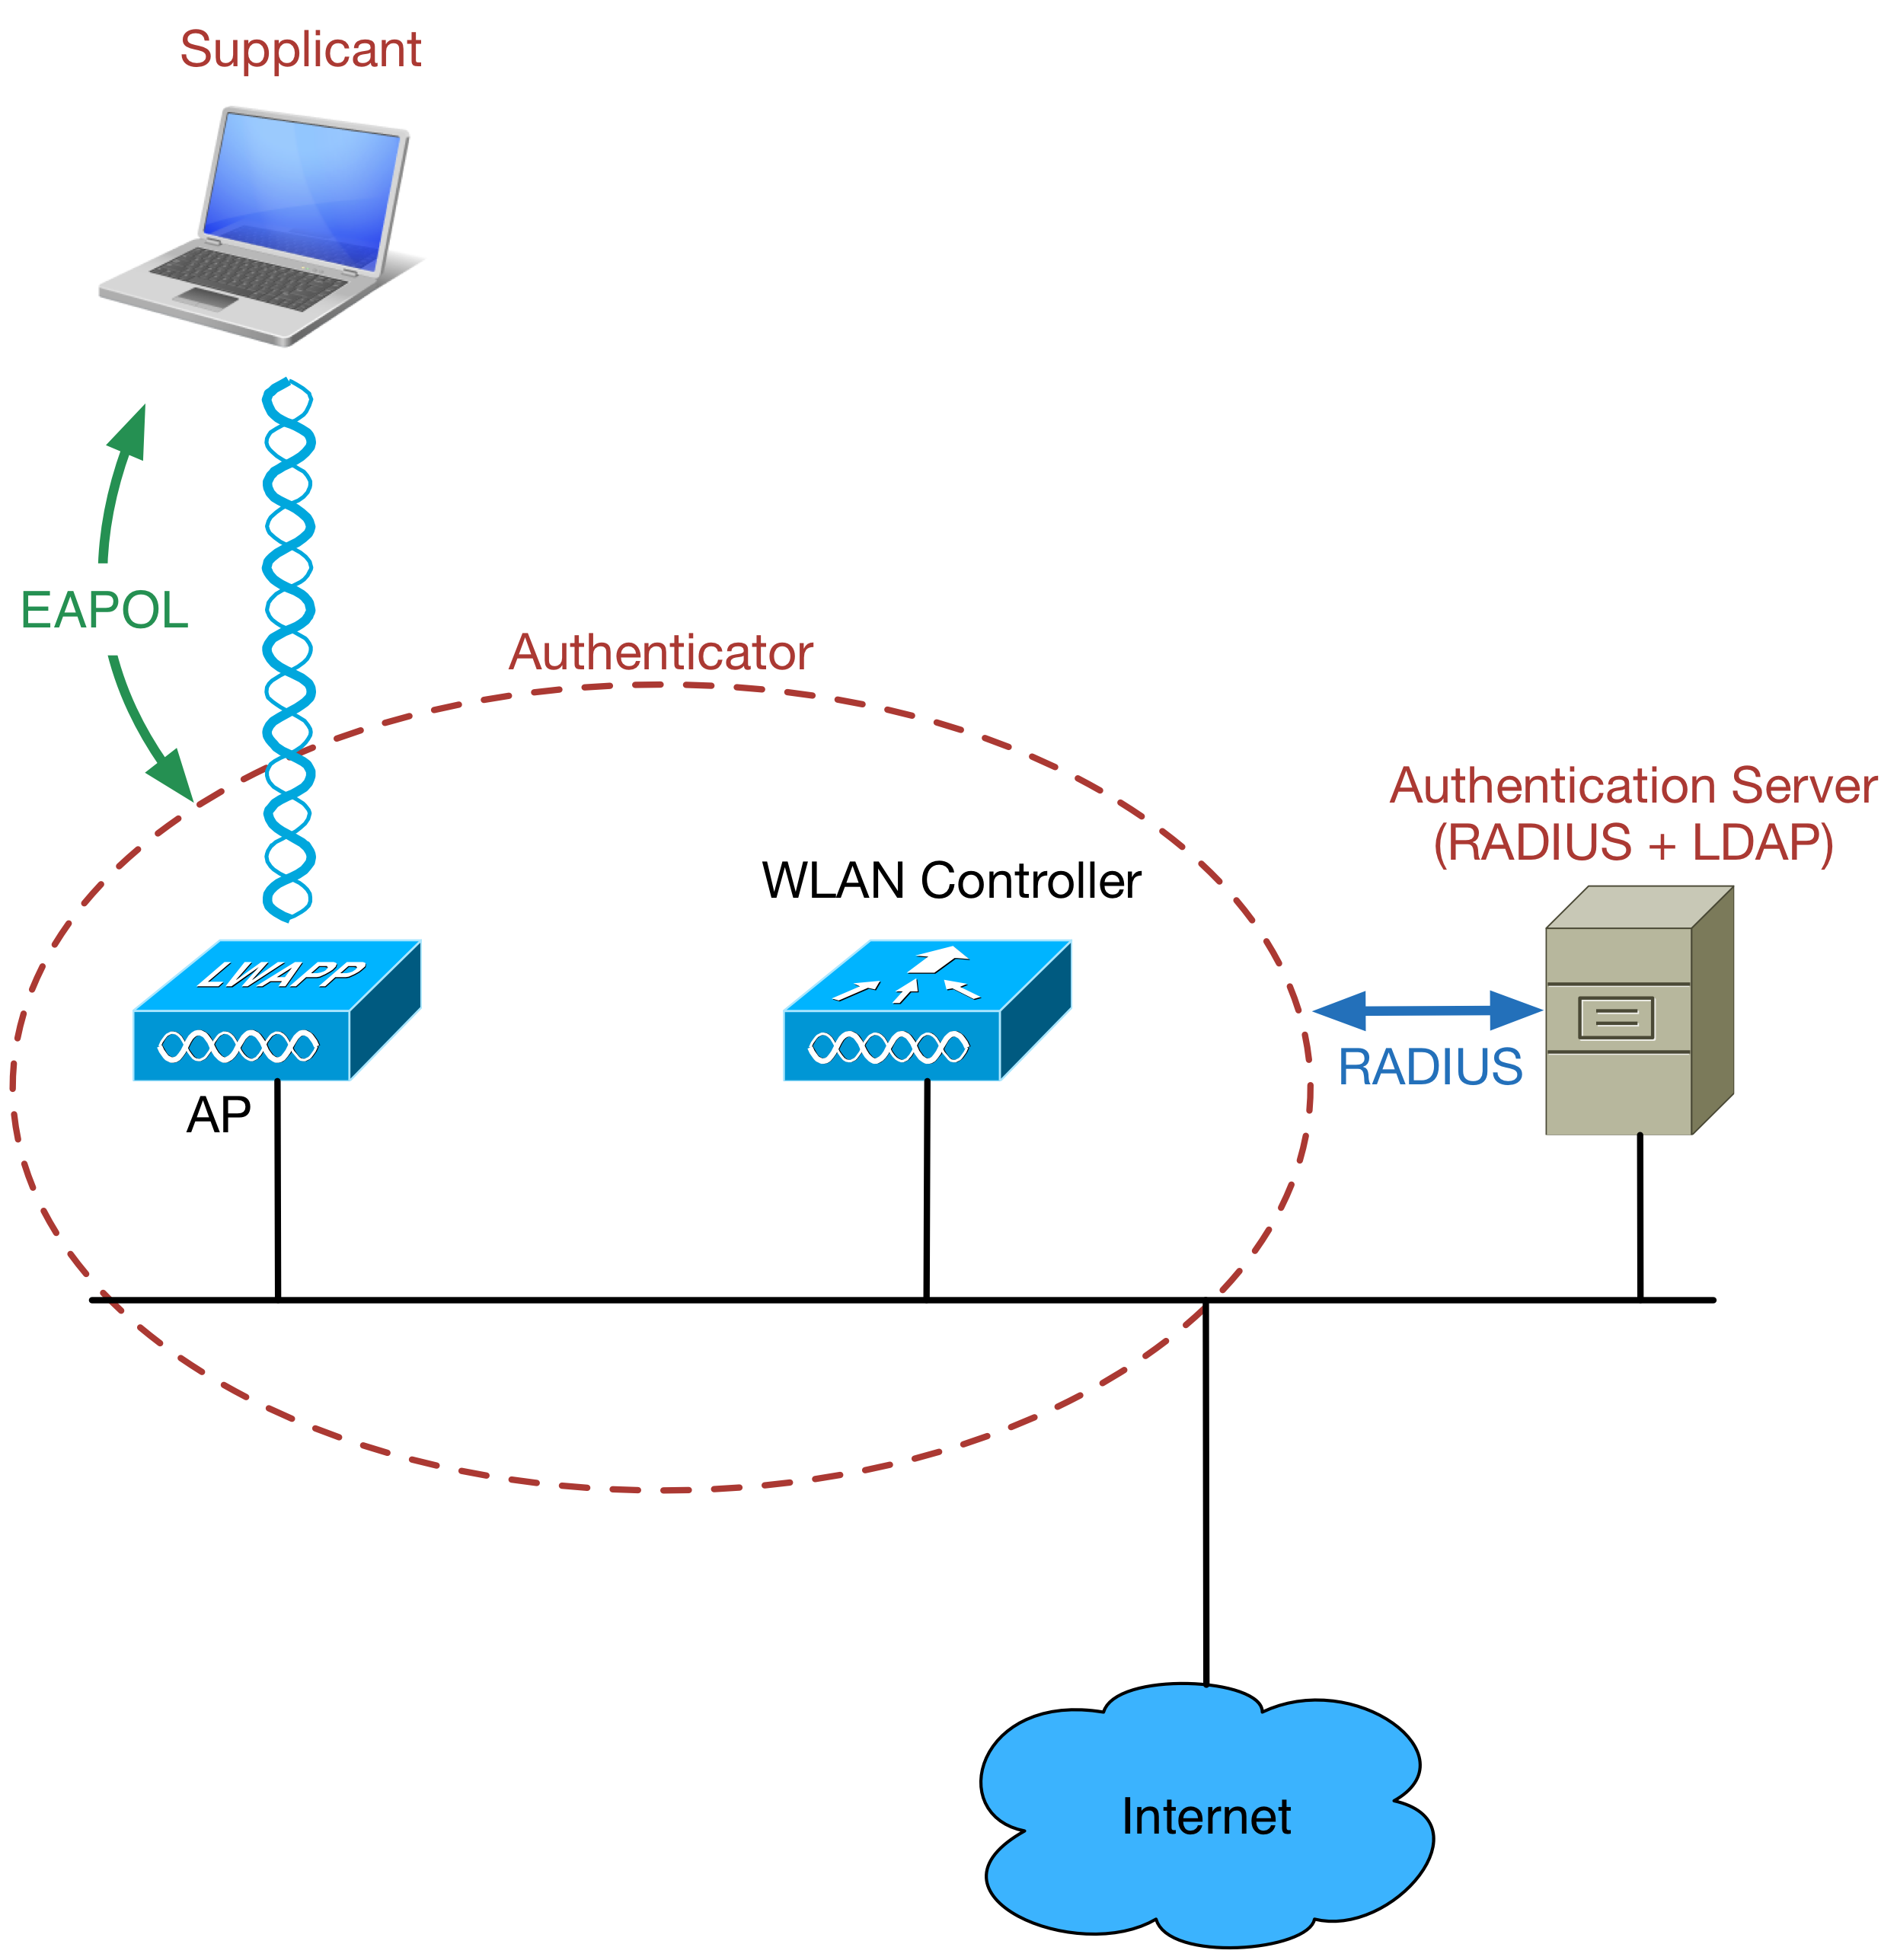
\includegraphics[width=.9\linewidth]{Pictures/Chapter2/topology.png}
	\caption{Authentication process on a UCL's WLANs}
\end{figure}


\subsection{student.UCLouvain authentication example}
To illustrate how the whole authentication process works, let's take a closer look to what happens when a student wants to connect to the \texttt{student.UCLouvain} network.
As detailed above, this network is protected by the \texttt{802.1X} authentication protocol. Thus the client first needs to authenticate himself before being able to access the Internet.
As a reminder, the client who wants to connect the network is called the \textit{supplicant}. This supplicant is going to first make a standard \texttt{802.11} association with the authenticator. The authenticator is composed of the access point to which the supplicant is trying to connect and the WLAN controller that is going to handle the whole authentication request. Once this association has been made, the authenticator understands that the supplicant wants to get an access to the protected network and thus a \texttt{802.1X} session between them is started. At this state, only \texttt{802.1X} traffic is allowed (i.e. only \texttt{EAP} messages are accepted during the transmissions).

The first message the supplicant is going to send to the authenticator is an \texttt{EAPOL-Start} frame in order to initiate the authentication process. When the authenticator receives that frame, it sends an \texttt{EAP-Request Identity} frame to the supplicant that answers with an \texttt{EAP-Response Identity} frame containing the supplicant's identity. The authenticator encapsulates this response in a \texttt{RADIUS Access-Request} packet and forwards it to the authenticator server.

Once the authentication server has received that packet it sends a \texttt{RADIUS Access Challenge} back to the authenticator containing an \texttt{EAP Request} specifying the type of \texttt{EAP} method to use (\texttt{TTLS} or \texttt{PEAP}) in order to validate the identity of the supplicant and to specify how the credentials are submitted. The authentication server also sends its certificate during that negotiation. The authenticator encapsulates that \texttt{EAP Request} in an \texttt{EAPOL} frame and sends it to the supplicant.

Since the supplicant has a copy of the server certificate, it can checks if the one received during the negotiation is the same in order to authenticate the server's identity. Once its identity has been proved, the supplicant builds a \texttt{TLS-encrypted} tunnel with the authentication server. It then sends its credential securely inside this channel.

The authentication server validates the username and password of the supplicant and sends back a \texttt{RADIUS Access-Accept} packet to the authenticator that sends an \texttt{EAP-Success} frame to the supplicant. The authenticator opens the port for the supplicant and by doing so, completing the process of authentication and allowing the user to access the Internet after having negotiated a \texttt{WPA} key with the authenticator.

The following figure represents the main steps of the authentication process for the \texttt{student.UCLouvain} network:

\begin{figure}[H]
	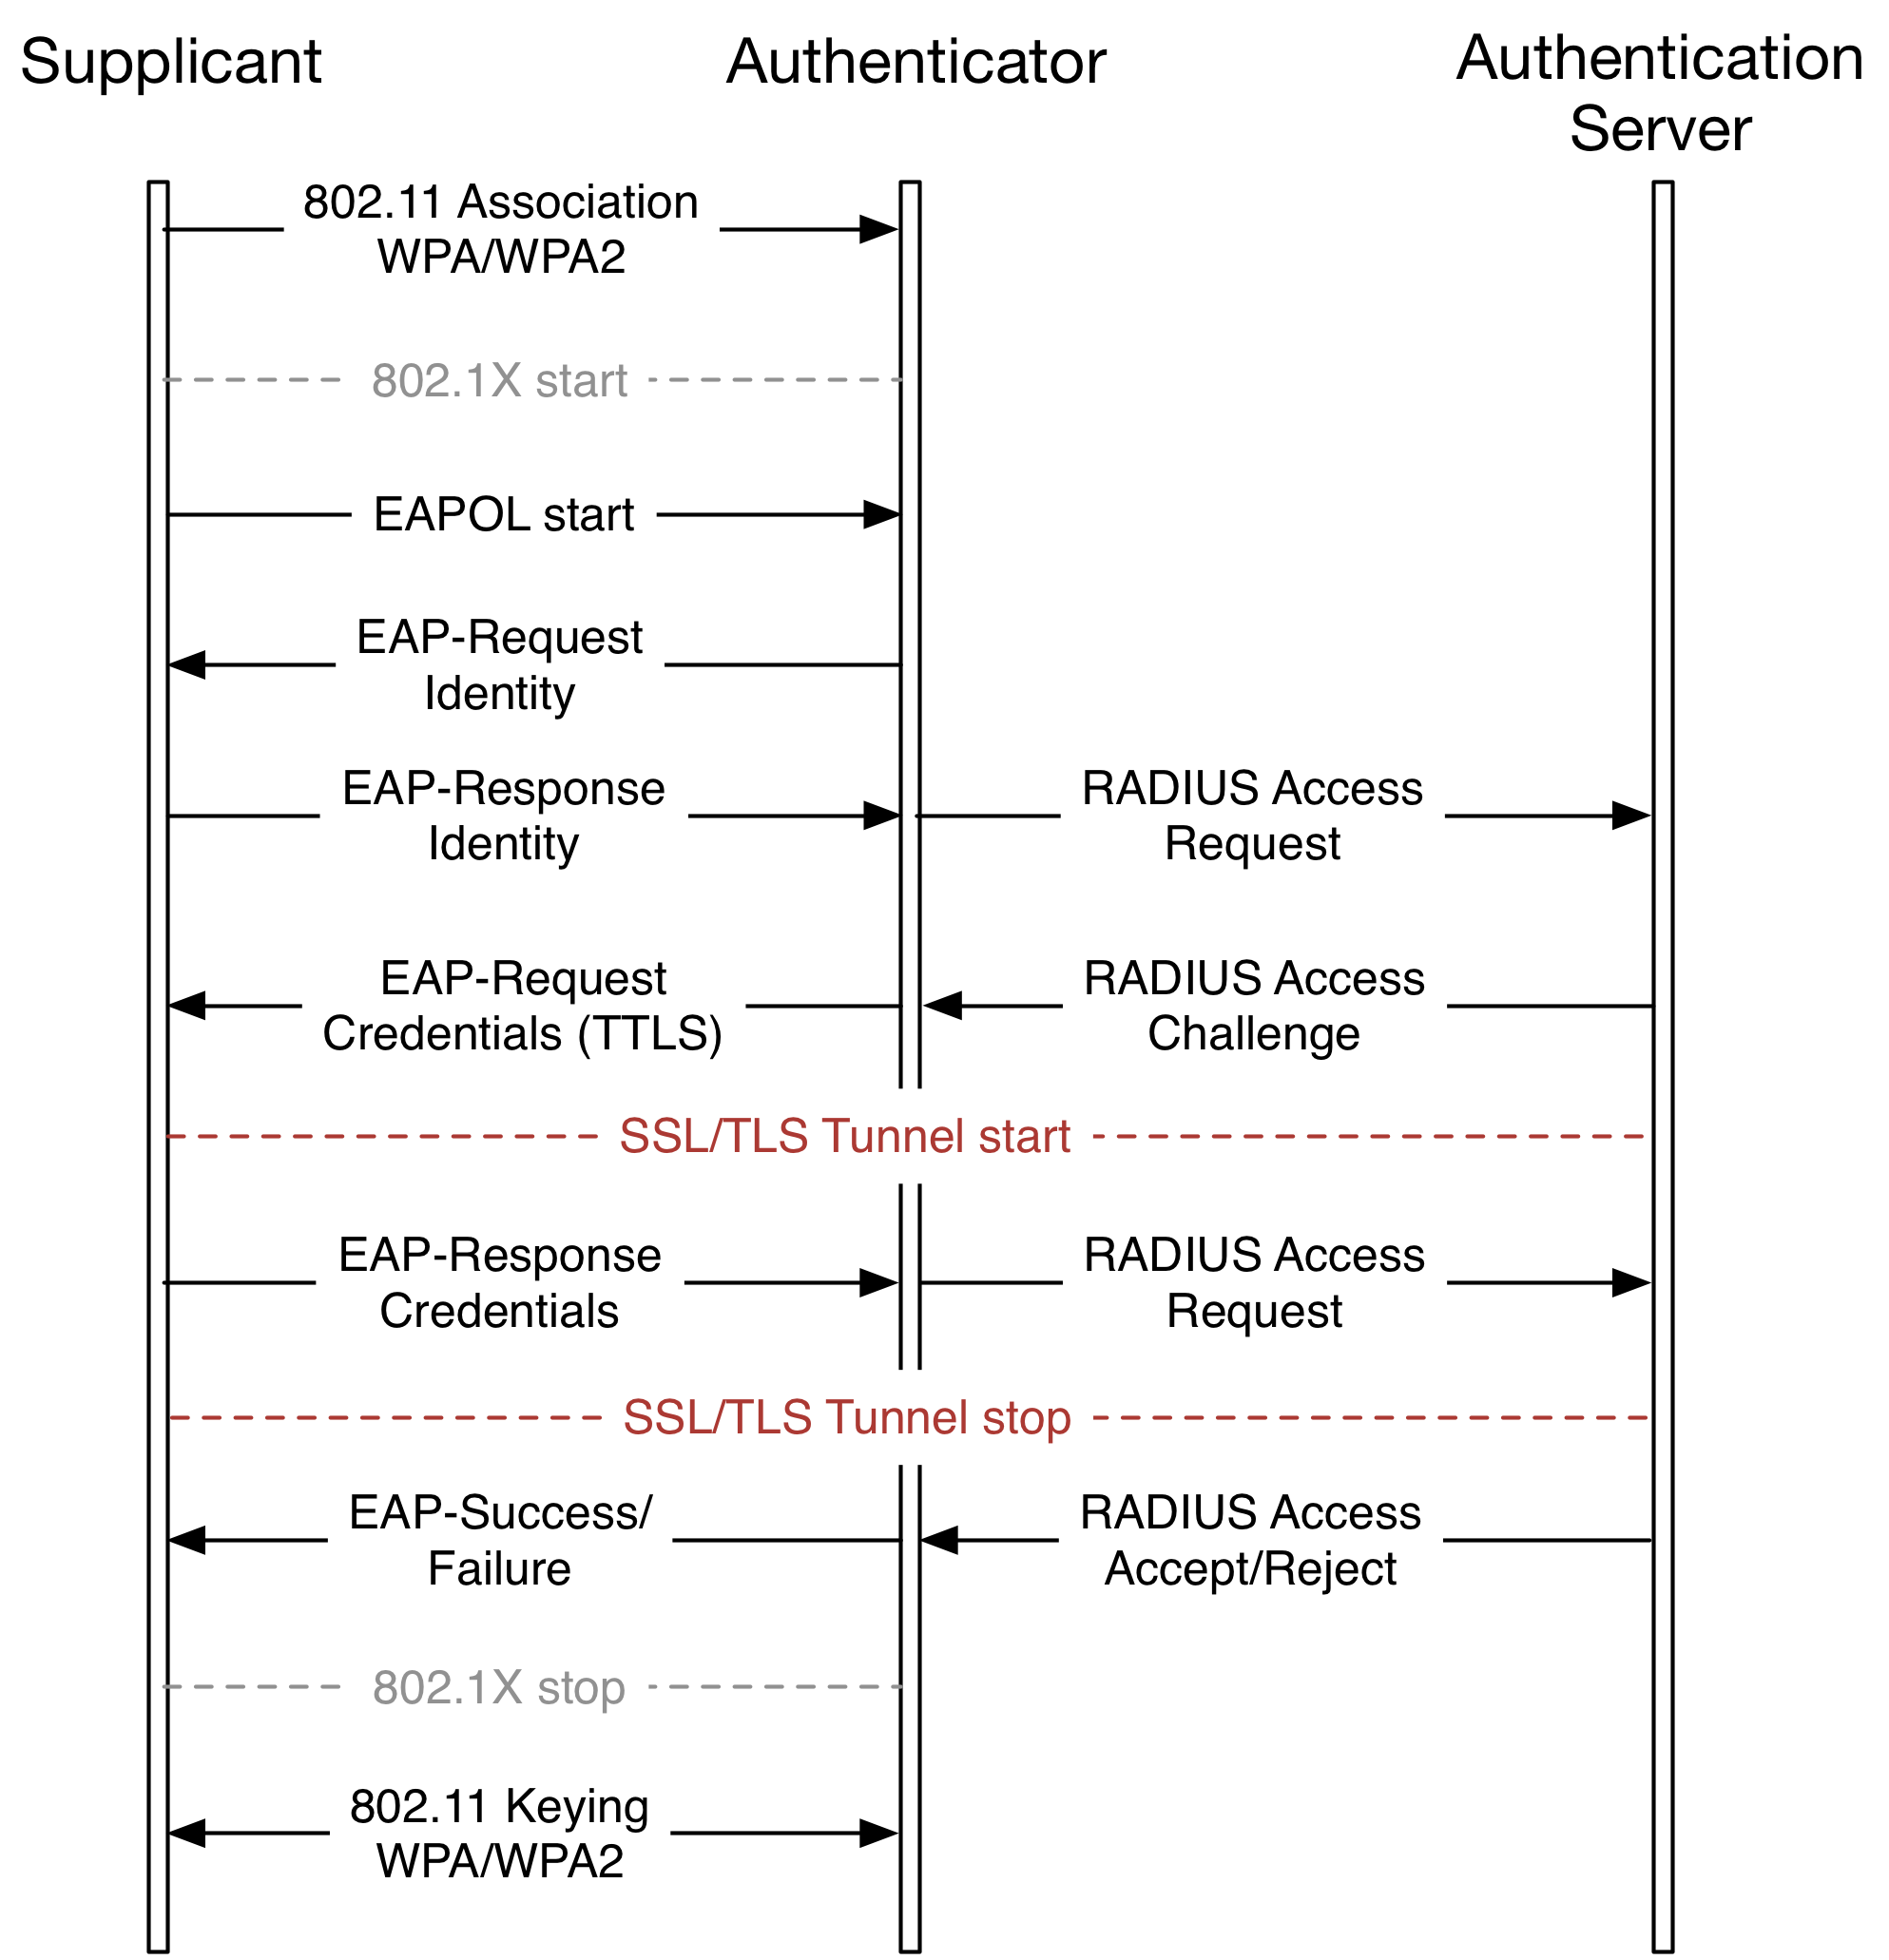
\includegraphics[width=.9\linewidth]{Pictures/Chapter2/student.png}
	\caption{student.UCLouvain authentication process}
\end{figure}


\subsection{eduroam authentication example}
Let's take another WLAN authentication process example with the \texttt{eduroam} network which is a bit different than the example seen before.
As explained in \cite{eduroamRadius}, the \texttt{eduroam} project is "\textit{A wolrdwide federation of} \texttt{RADIUS} \textit{ servers facilitating network access for roaming academic affiliates using} \texttt{IEEE 802.1X} \textit{as the vehicle. eduroam's use of} \texttt{802.1X} \textit{in concert with} \texttt{RADIUS} \textit{means the network is built around well understood, established, and easy to manage standards which are often already deployed within the network infrastructure of educational institutions}".

Since \texttt{eduroam} is also using the \texttt{802.1X}, when a client want to connect to the network, he is not able to pass any traffic other than \texttt{802.1X} until his request is accepted by the authentication server. As for the \texttt{student.UCLouvain} network, the communication between the supplicant and the authenticator also involves \texttt{EAP} conversation.The supplicant sends its \texttt{EAP} messages to the authenticator that forwards them to the authentication server in the form of a \texttt{RADIUS} request. To ensure the protection of the credentials and information sent during the authentication negotiation, eduroam uses either \texttt{TTLS} or \texttt{PEAP} (\textit{Protected Extensible Authentication Protocol}).A \texttt{TLS-encrypted} tunnel is also created between the supplicant and the authentication server.

As a student from another university than the Catholic University of Louvain can access and connect to the \texttt{eduroam} network from inside the Louvain-la-Neuve campus, the local authentication server, in Louvain-la-Neuve, is not the one that is going to handle the authentication request. Indeed, if the user comes from a given university in Spain, for example, its authentication request will be forwarded to the Belnet \texttt{RADIUS} server that will forward the request to the authentication server of the student's university. The \texttt{RADIUS} protocol supports that forwarding in its proxy mode. To prevent any administrators not responsible for the handling of the authentication request, the \texttt{TLS-encrypted} tunnel is propagated throughout the \texttt{RADIUS} infrastructure. Thanks to that tunnel, the intermediate authenticator does not handle sensitive information during the authentication process.

Here is a representation of the authentication request communications between the supplicant, the authenticator and the authentication server with \texttt{RADIUS} proxying:
\begin{figure}[H]
	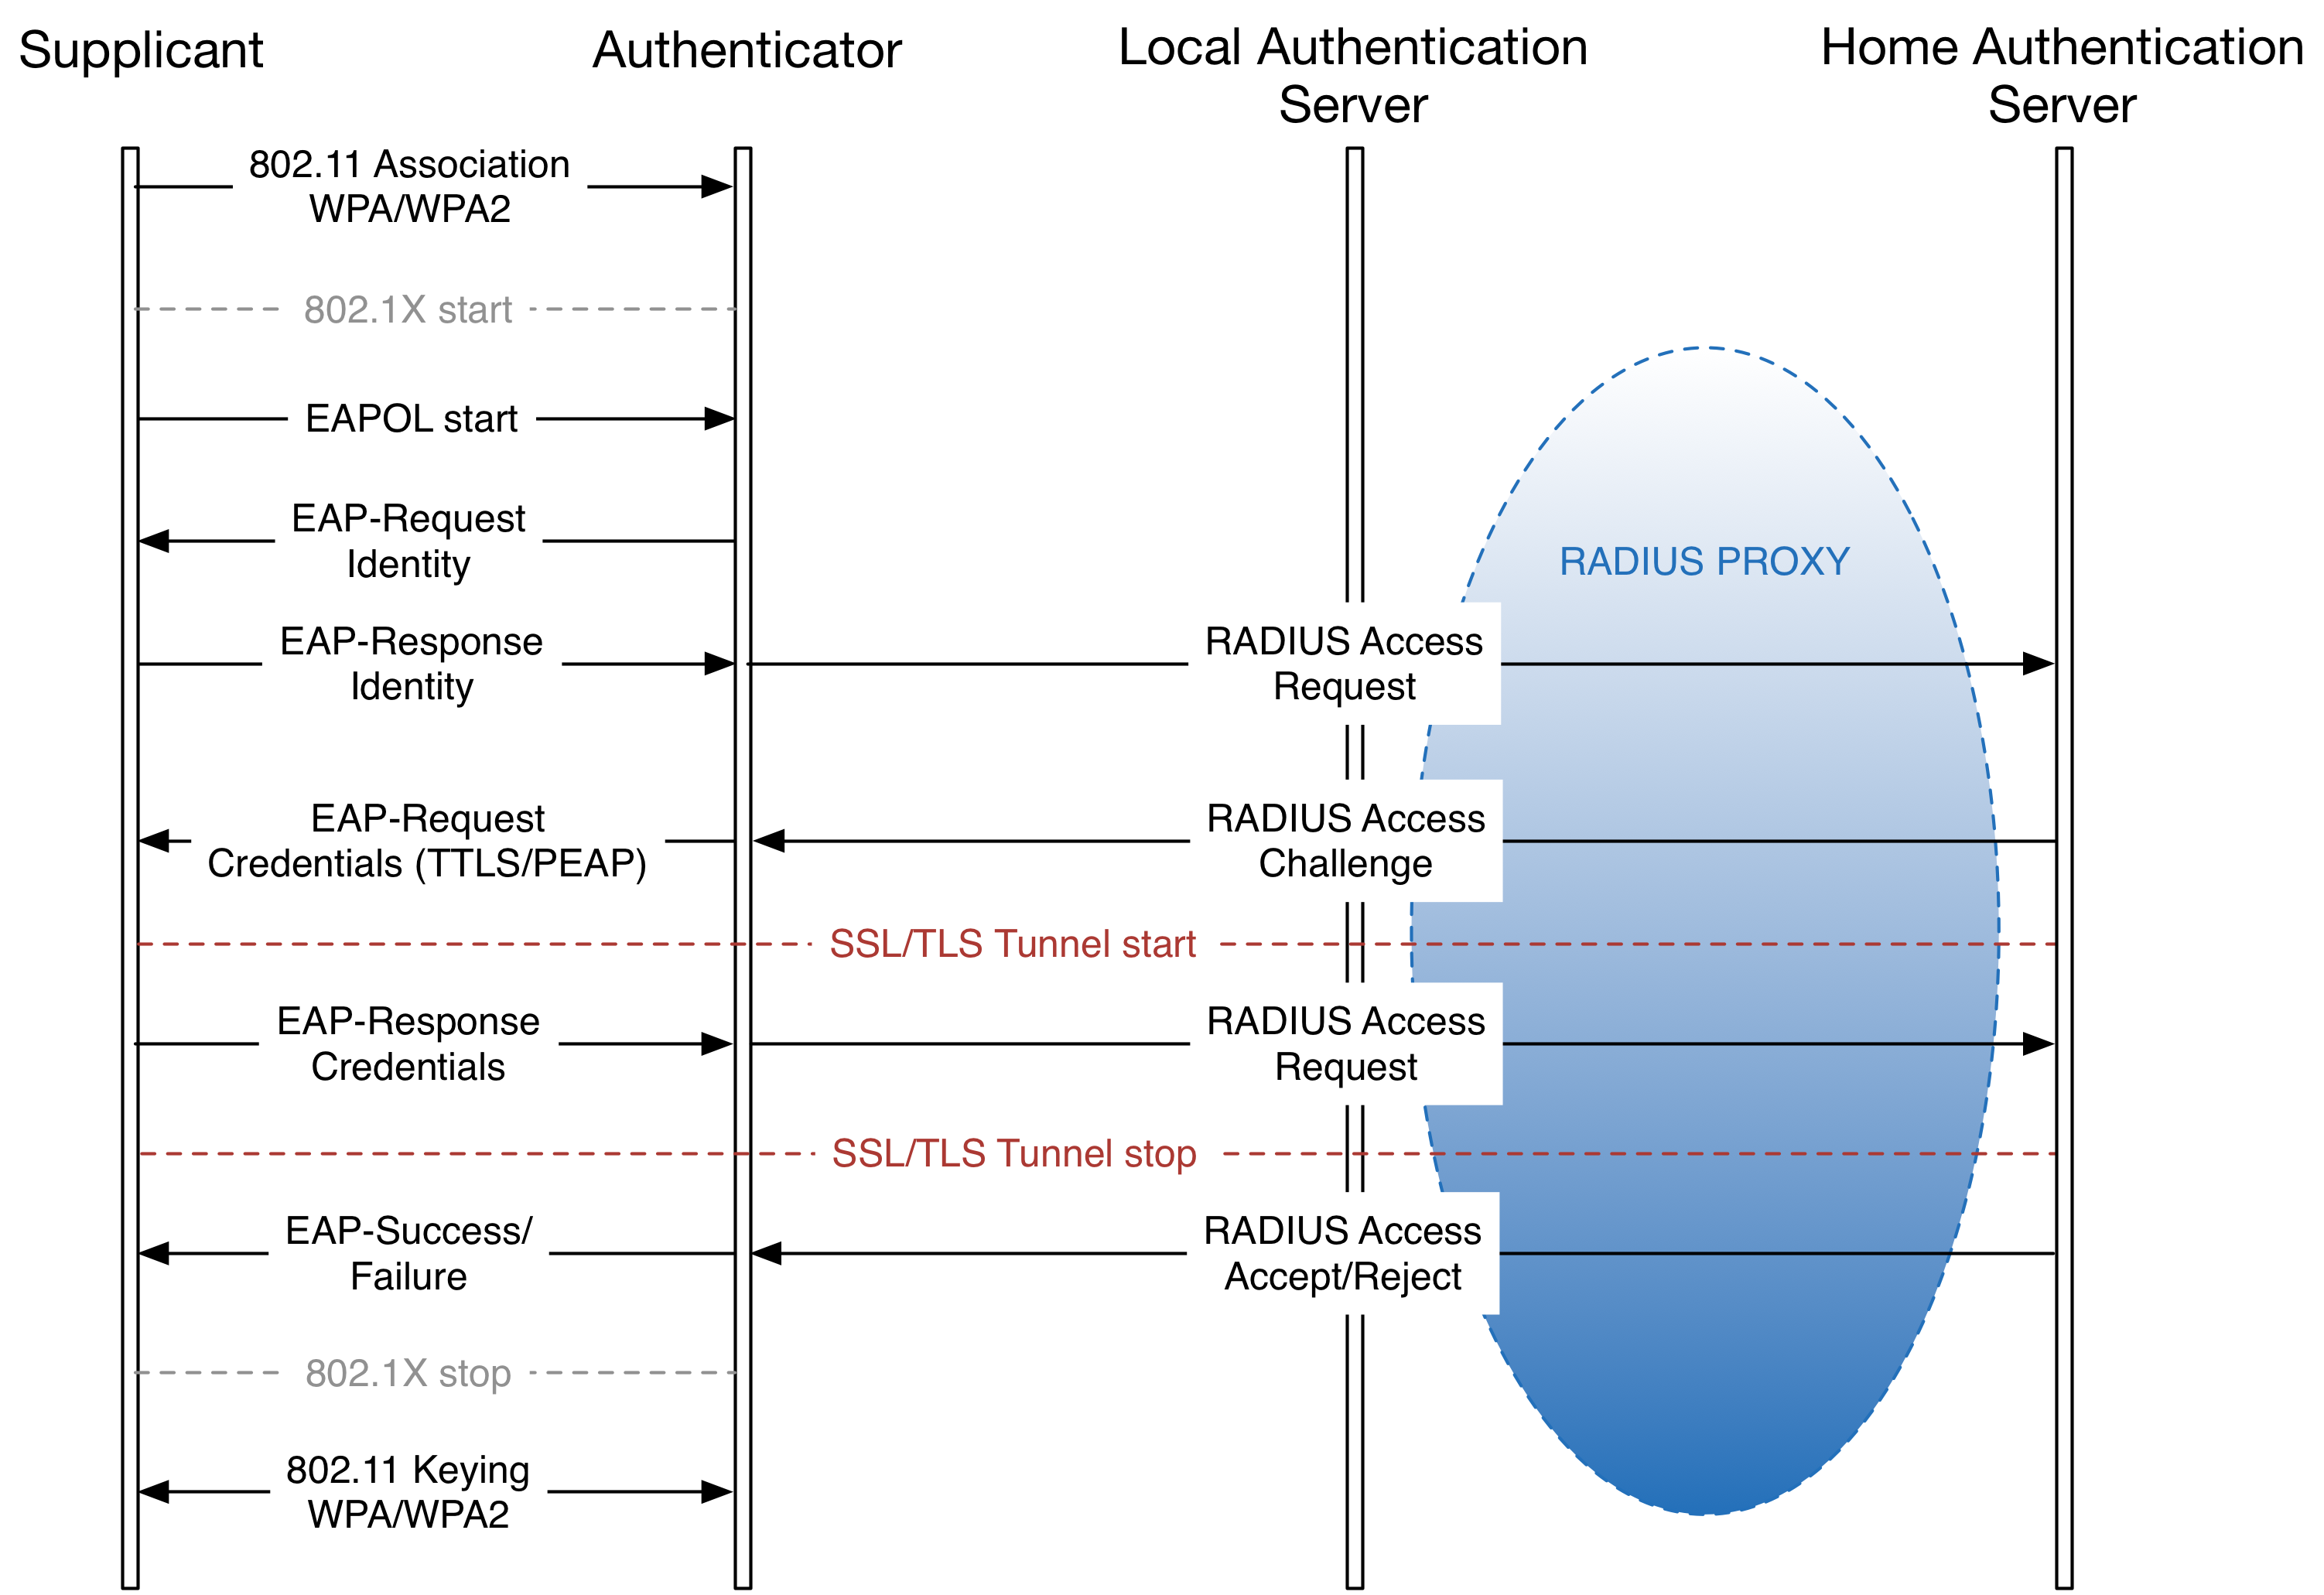
\includegraphics[width=1\linewidth]{Pictures/Chapter2/eduroam1.png}
	\caption{eduroam authentication process}
\end{figure}


\section{LAN authentication process}
%http://www.resinfo.cnrs.fr/IMG/pdf/josy.07.mobilite.borderes.radius.pdf
The Catholic University of Louvain also provides a wired connection to the different networks.

In order to do so, the user's computer needs to be first added to the allowed clients database. This database stores all the MAC addresses that are allowed to access to the networks. 
To be able to add his computer MAC address, the user needs to be enrolled at the university and to prove it by giving is \texttt{NOMA} (i.e. member ID), his university's username and email.

The protocol used here is a bit different and is called \texttt{RADIUS-MAC}. With this protocol, the supplicant directly plugs into the switch (1). The switch detects the connection and sends an authentication request (2) to the \texttt{RADIUS} server with the MAC address of the supplicant as identifier. The server then checks in his database if the MAC address is allowed on the network or not. If the address is known, the server sends back (3) an \texttt{Access-Accept} response to the authenticator that opens the port for the supplicant that has now a full access (4) to the protected network. The following figure shows all the steps in this process.

\begin{figure}[H]
	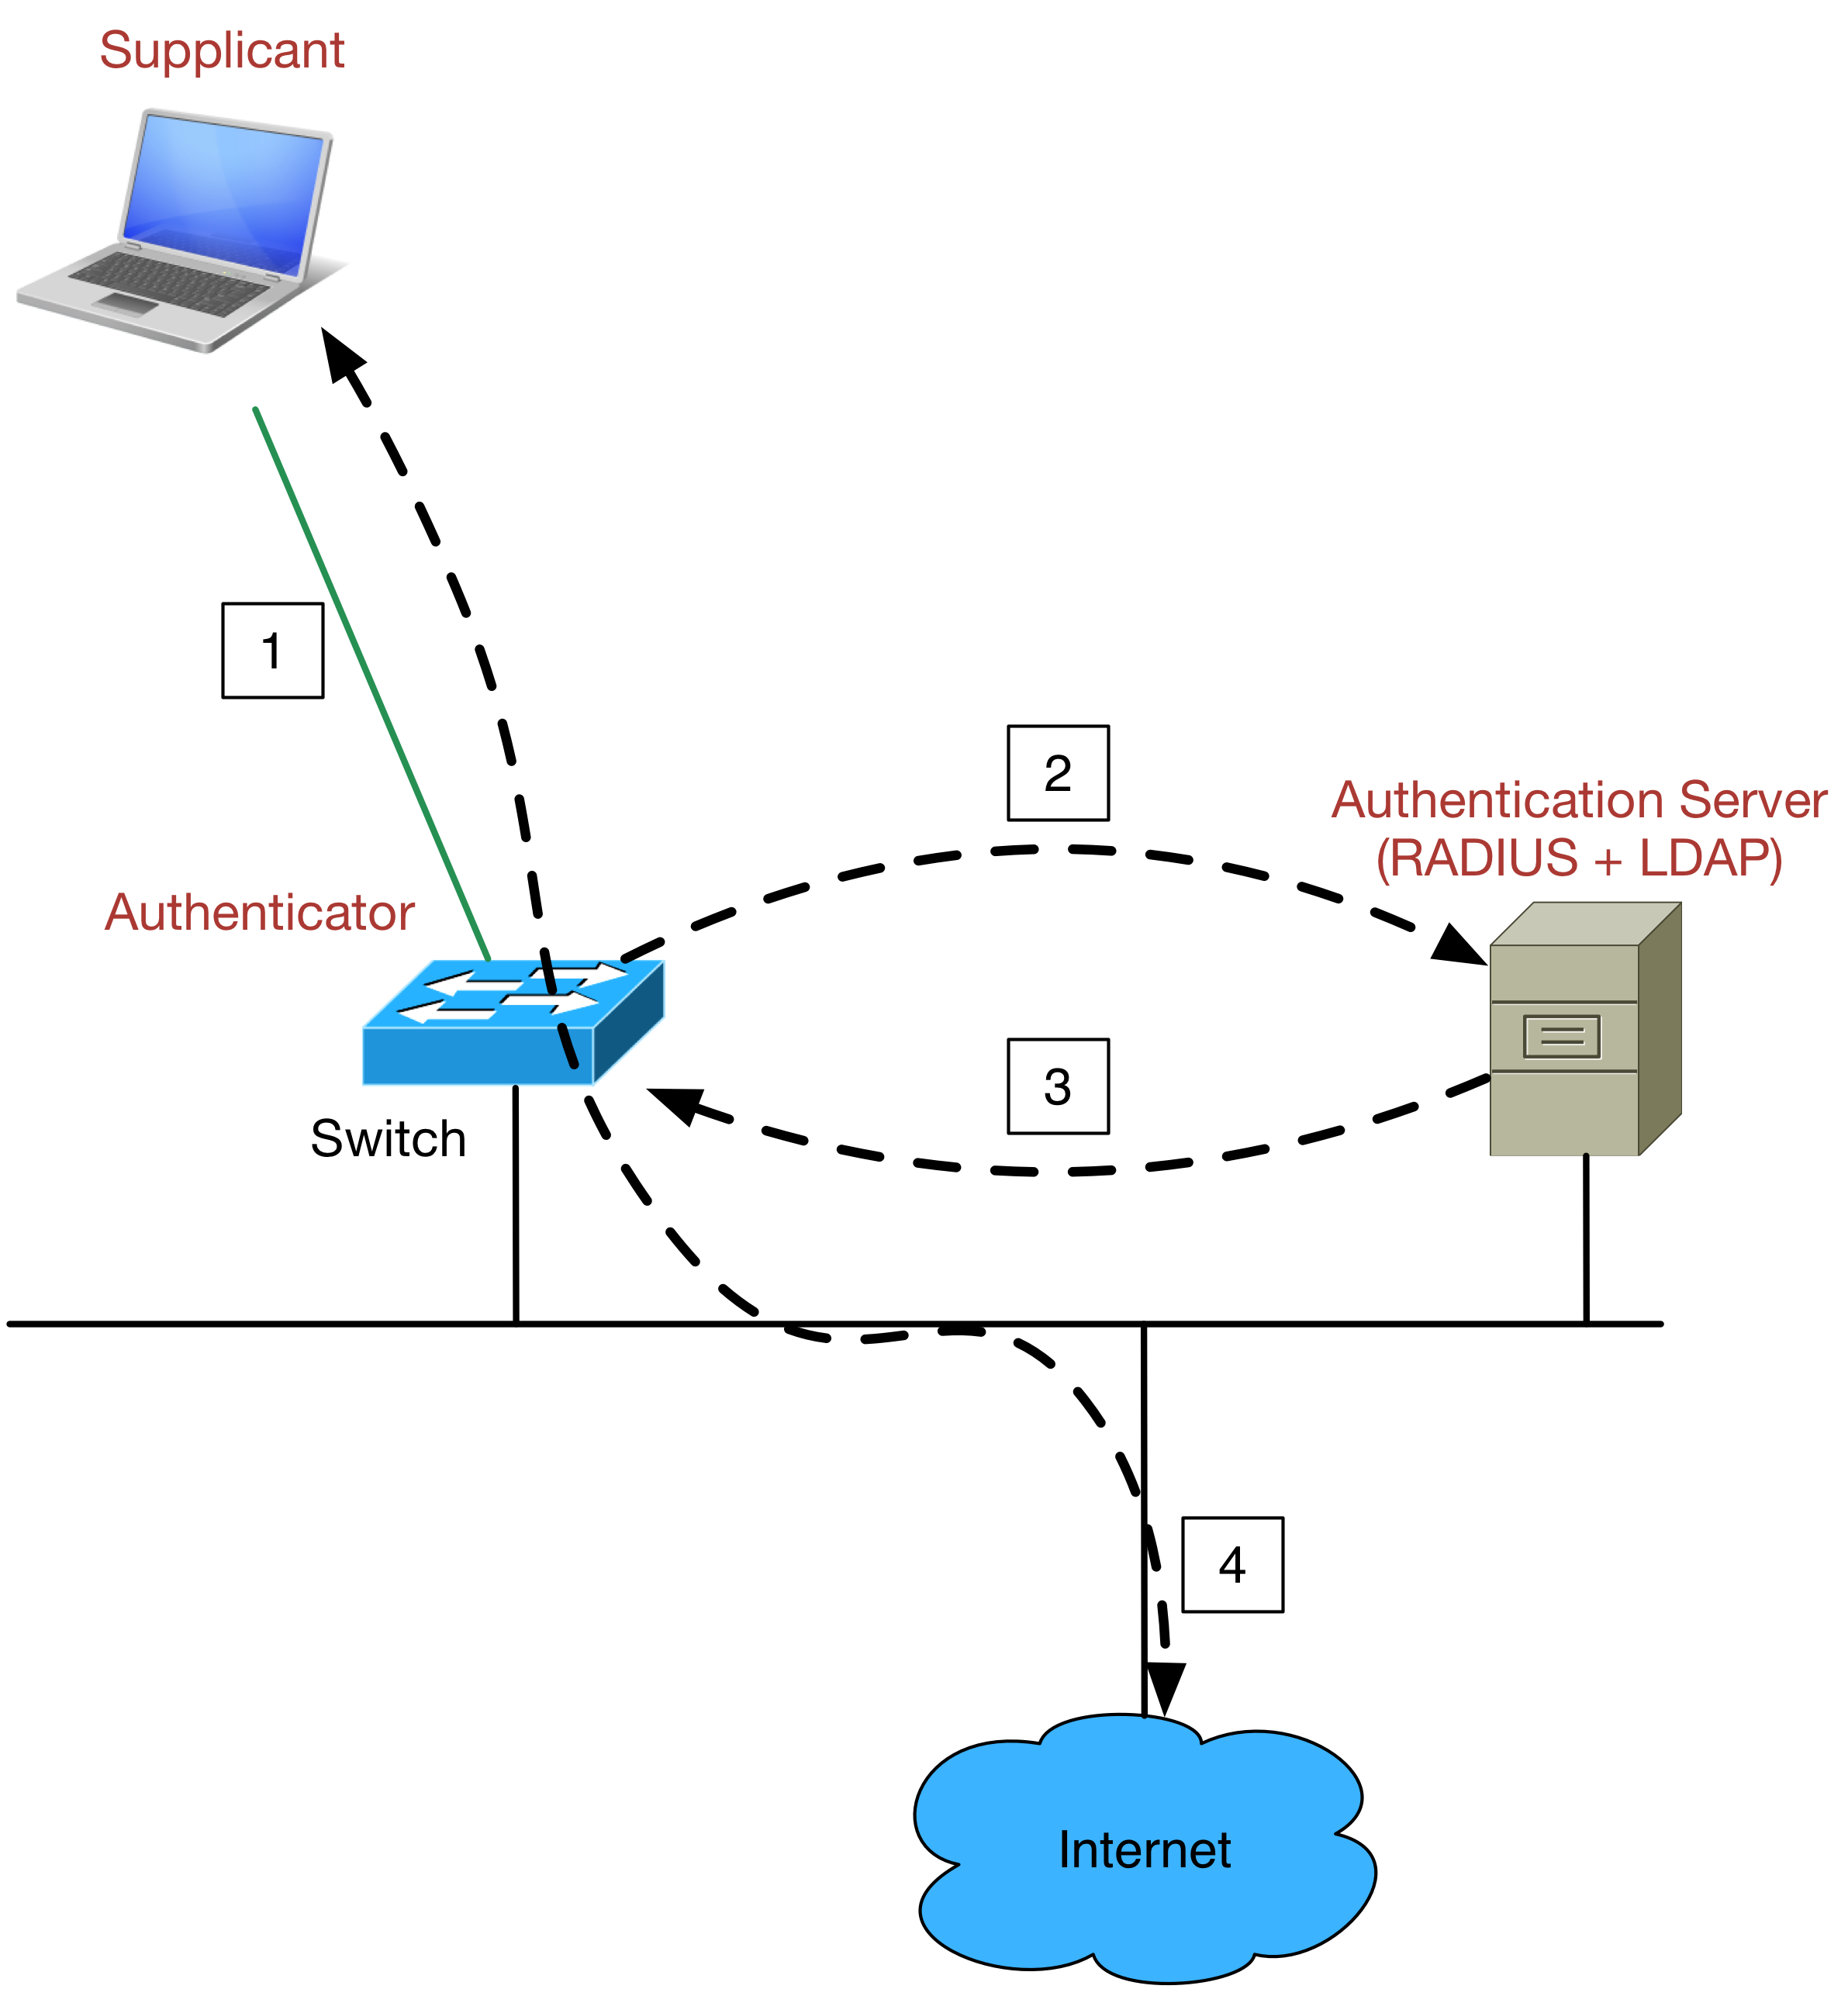
\includegraphics[width=.7\linewidth]{Pictures/Chapter2/wired.png}
	\caption{Authentication process on a UCL's LANs}
\end{figure}

Since our thesis is about a monitoring tool for the WLANs of the Catholic University of Louvain, we won't go in any further details concerning the LAN security management. 
Still we have given a little overview of the LAN authentication process because we think it is important to know that this process also exists within the university's network infrastructure.


\section{Infrastructure architecture}
Within the Catholic University of Louvain's network infrastructure architecture, the Internet access is provided by Belnet via a 10Gbit Ethernet link. This link is connected to one of the seven \textit{neighborhood routers} called \texttt{CtPythagore}. There is also a second 1Gbit Ethernet link connected to another neighborhood router called \texttt{CtHalles}. This second link is never used and is, in fact, a backup link in case of a failure of the main one.

The other neighborhood routers are \texttt{CtLew}, \texttt{CtStevin}, \texttt{CtCarnoy}, \texttt{CtMichotte} and \texttt{CtSHI1C}. They are all on the Louvain-la-Neuve campus expect for \texttt{CtLew} that lies on the Woluwe campus in Brussels. Those neighborhood routers are all \texttt{Cisco Catalyst 6509} switches and are the campus core routers. Two of them (\texttt{CtSH1C} and \texttt{CtMichotte}) include a \texttt{Cisco WiSM2} (\textit{Wireless Services Module 2}) controller. The infrastructure also contains two data centers called \texttt{CtTier2} and \texttt{CtAquarium}. Each one of those data center has a load balancer. The two \texttt{DHCP} servers as well as the \texttt{LDAP} servers are located behind those load balancers.

Here is a representation of the UCL's network infrastructure.

\begin{figure}[H]
	
\includegraphics[width=1\linewidth]{Pictures/Chapter2/ucl.png}
	\caption{UCL's network infrastructure architecture}
\end{figure}


Each building on the Louvain-la-Neuve campus has a direct connectivity with the network. Inside there are several access points (either \texttt{Cisco Aironet 3600} or \texttt{Cisco Aironet 3700}) that provide an Internet access to the clients and also a patch room that contains some \texttt{Cisco Catalyst 2960S-48LPS} switches to which the access points are connected. The network, and thus the controllers, is connected to the patch room allowing communications between the network infrastructure and the clients.

The following figure represents a simplified overview of how the buildings are connected to the network.

\begin{figure}[H]
	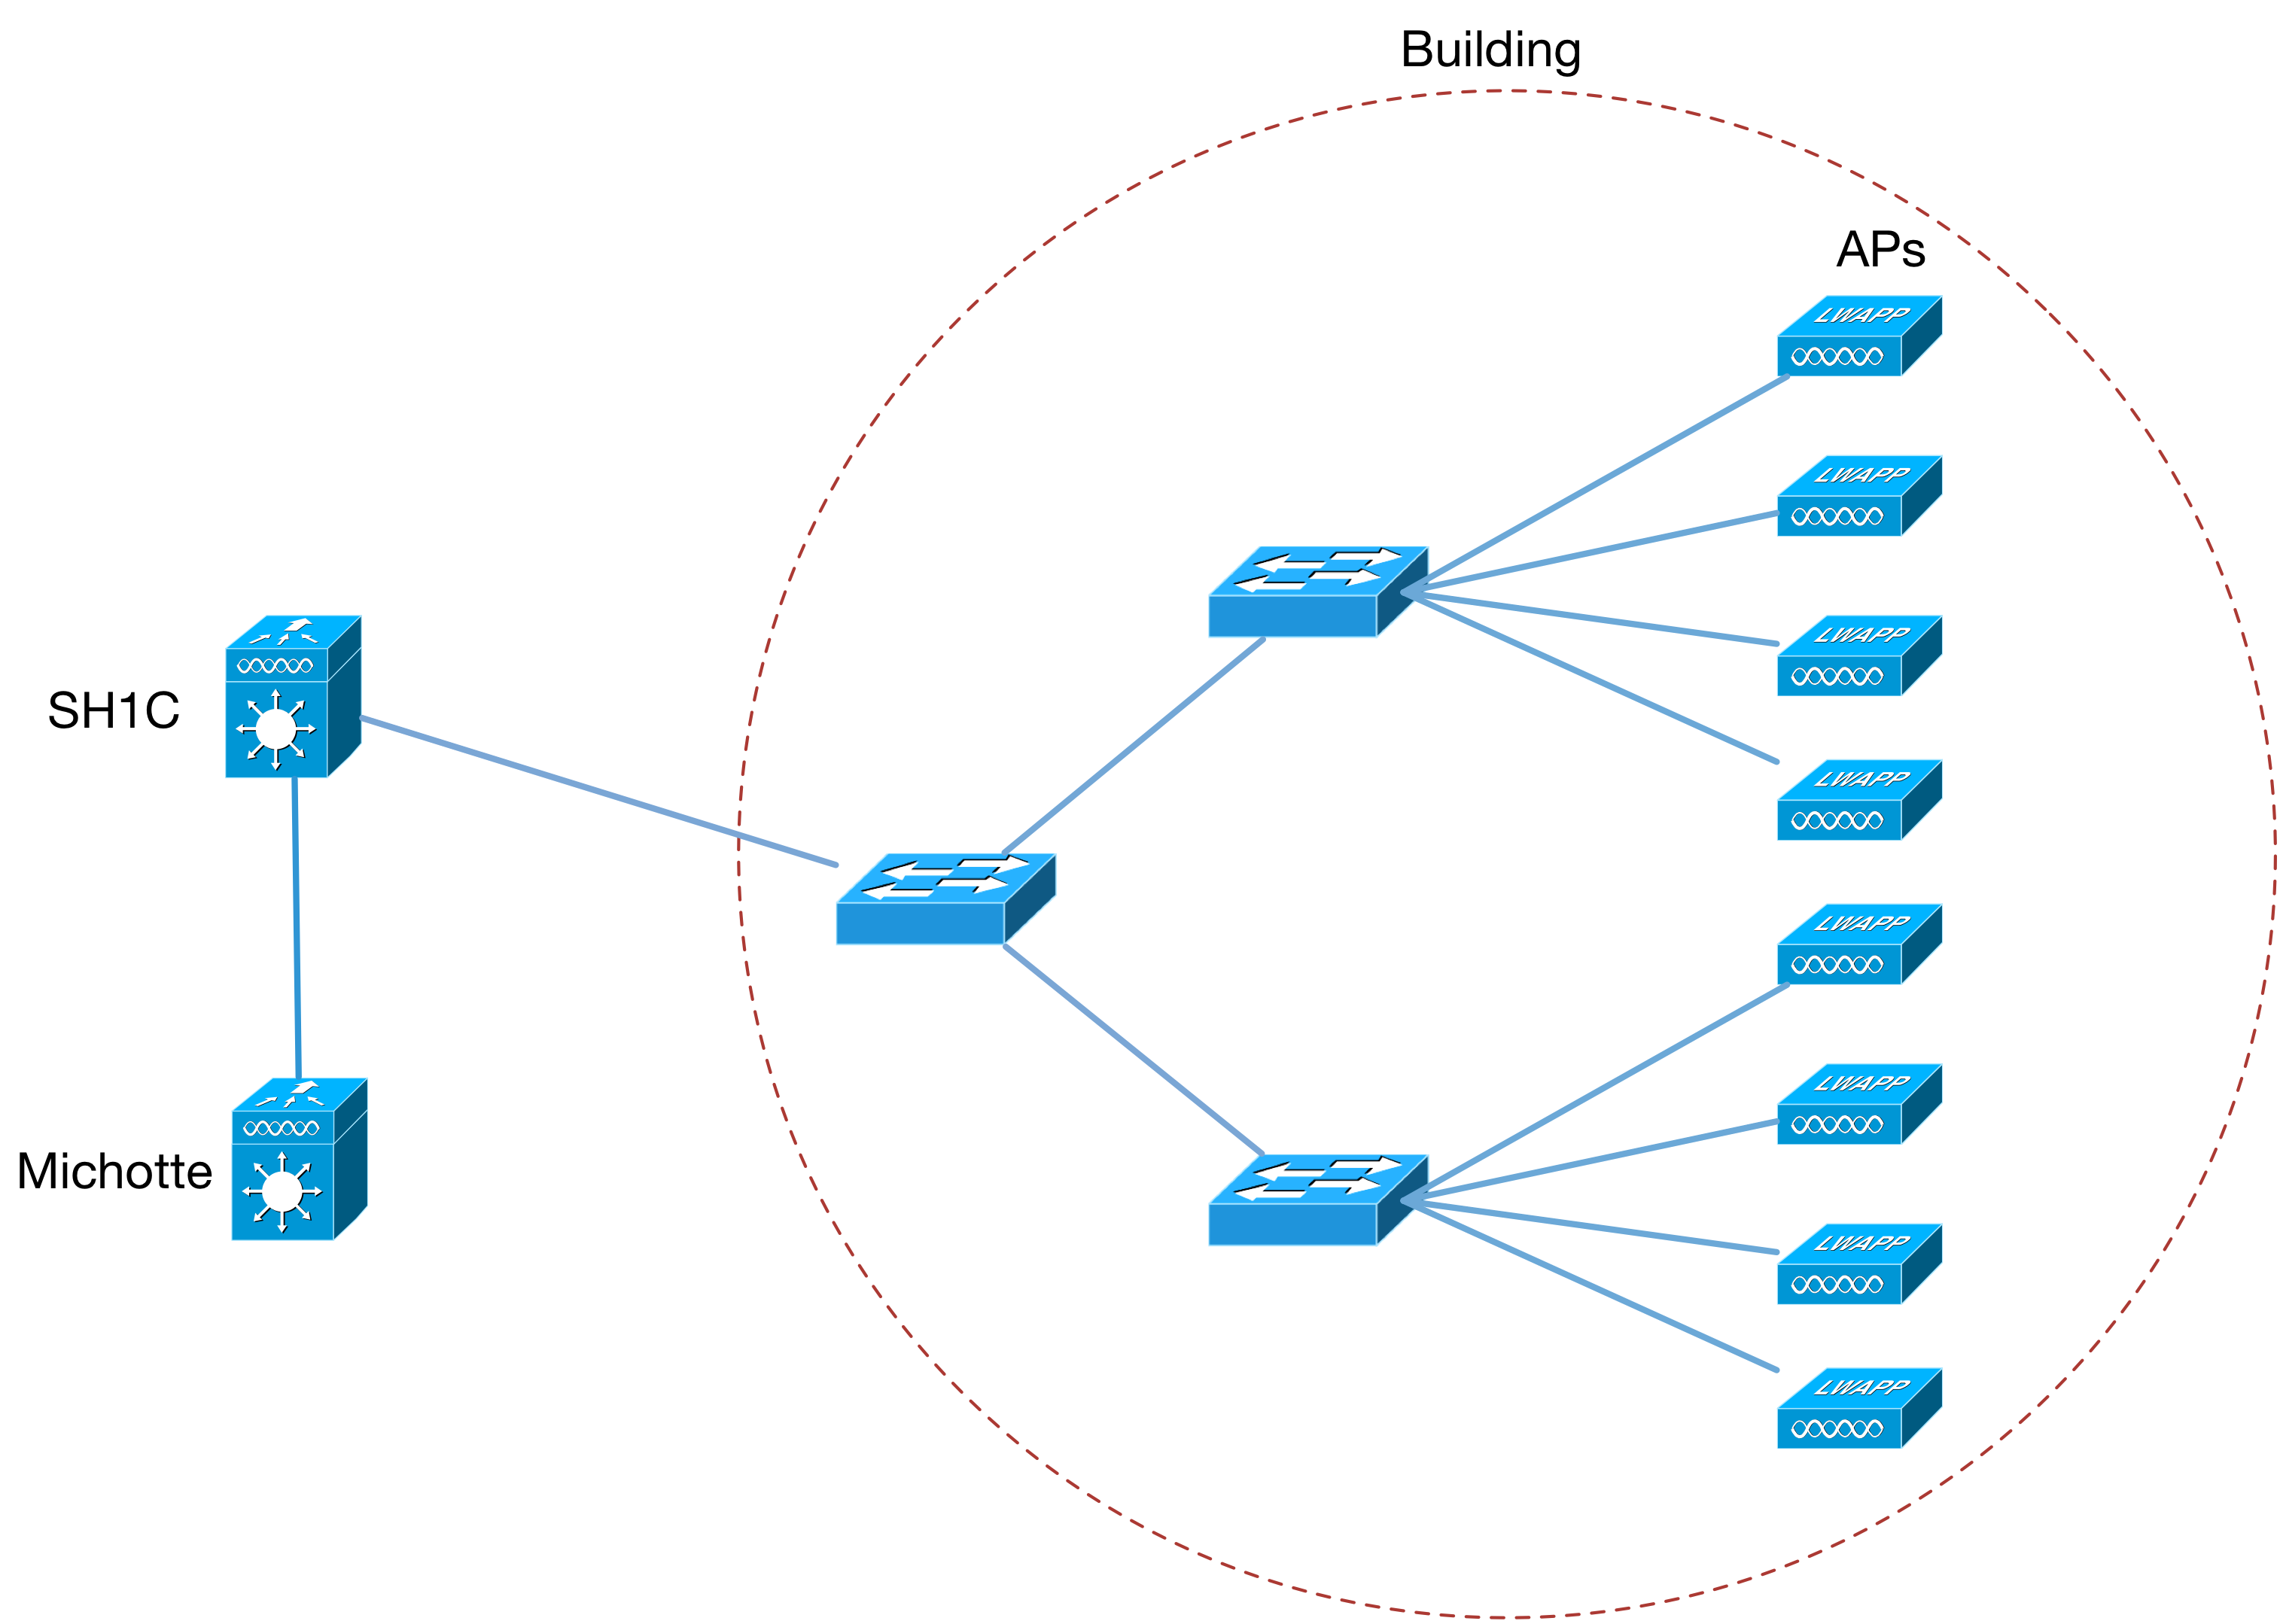
\includegraphics[width=1\linewidth]{Pictures/Chapter2/building.png}
	\caption{Building infrastructure and network connection}
\end{figure}

%TODO
%Here is a simplified representation of the UCL network infrastructure:
%\begin{figure}[H]
%	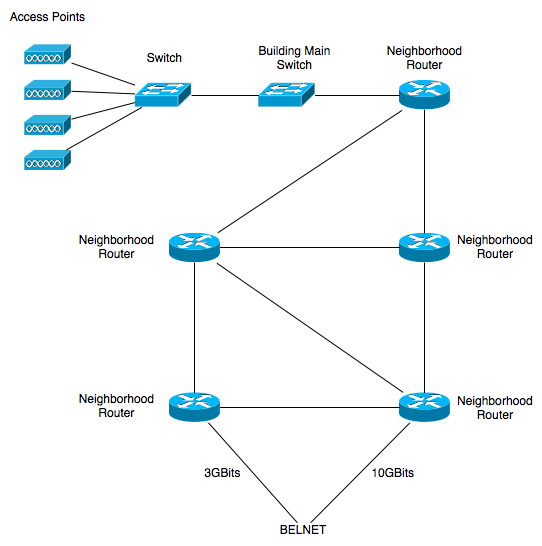
\includegraphics[width=.9\linewidth]{Pictures/Chapter2/infrastructure.png}
%\end{figure}



